% G-SYMBOL-03: selected A2, B1 and D1, normalized to width = 25 wire strokes.
% All dimensions use stroke centre lines. Stem length is W for these samples.
\documentclass{article}
\usepackage[paperwidth=7.2cm,paperheight=2.5cm,margin=0pt]{geometry}
\pagestyle{empty}
\setlength{\parindent}{0pt}
\usepackage{fontspec}
\IfFontExistsTF{TeX Gyre Heros}{\setmainfont{TeX Gyre Heros}}{\setmainfont{Arial}}
\usepackage{tikz}
\newdimen\GroundWidth
\newcommand{\GroundSymbol}[1]{%
  \begin{scope}[x=\GroundWidth,y=\GroundWidth]
    \draw (0,1)--(0,0);
    \ifnum#1=0
      \draw (-0.5,0)--(0.5,0);
    \else\ifnum#1=1
      \draw[fill=none] (-0.5,0)--(0.5,0)--(0,-0.5)--cycle;
    \else
      \draw (-0.5,0)--(0.5,0)
            ({-1/3},{-1/6})--({1/3},{-1/6})
            ({-1/6},{-1/3})--({1/6},{-1/3});
    \fi\fi
  \end{scope}}
\begin{document}
\noindent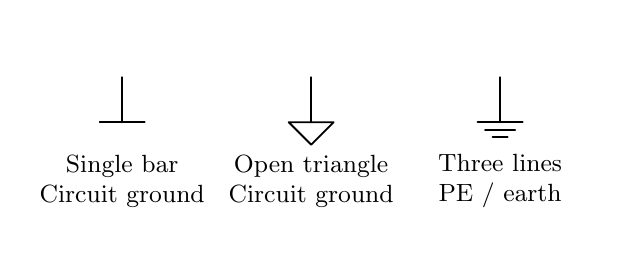
\begin{tikzpicture}[x=1cm,y=1cm,line width=0.65pt,
line cap=round,line join=round,font=\fontsize{9}{11}\selectfont]
\GroundWidth=25\pgflinewidth
\path[use as bounding box] (0,0) rectangle (7.2,2.5);
\begin{scope}[shift={(1.2,1.3)}]\GroundSymbol{0}\end{scope}
\begin{scope}[shift={(3.6,1.3)}]\GroundSymbol{1}\end{scope}
\begin{scope}[shift={(6.0,1.3)}]\GroundSymbol{2}\end{scope}
\node[align=center] at (1.2,0.55) {Single bar\\Circuit ground};
\node[align=center] at (3.6,0.55) {Open triangle\\Circuit ground};
\node[align=center] at (6.0,0.55) {Three lines\\PE / earth};
\end{tikzpicture}
\end{document}
